\documentclass[12pt]{iopart} % Document class declaration

% package "imports"
\usepackage{graphicx}
\usepackage{IEEEtrantools}
\usepackage{amsmath} % For centering equations

% Custom macros
\gdef\mcm{r@{.}l@{ ± }r@{.}l} % Multi Column Measurement; Used for decimal aligning & ± aligning
\gdef\mch#1{\multicolumn{4}{l}{#1}} % Multi Column Header; Used for decimal aligning & ± aligning
\gdef\mcmnd{r@{ ± }l} % Multi Column Measurement No Decimal; Used for ± aligning when the values don't need a decimal point
\gdef\mchnd#1{\multicolumn{2}{l}{#1}} % Multi Column Header No Decimal; Used for  ± aligning when the values don't need a decimal point
\gdef\sci#1#2{#1 \times 10^{#2}}
\gdef\units#1{~\mathrm{#1}}
\graphicspath{{./images/}}

%%%%%%%%%%%%%%%%%%%% Document Starts %%%%%%%%%%%%%%%%%%%%
\begin{document}

%%%%%%%%%%%%%%%%%%%% Title Page %%%%%%%%%%%%%%%%%%%%
\title{Realistic Projectiles}
\author{Ali Mortada, Xavier Valencia, James Phommachanh, Wes Cochran}
\vspace{10pt}
\begin{indented}
  \item[]Mt.~San Antonio College, ENGR 285, CRN 43464
  \item[]May 20, 2024
\end{indented}
\newpage

%%%%%%%%%%%%%%%%%%%% Objectives %%%%%%%%%%%%%%%%%%%%
\section{Objectives}

\begin{center}
\subtitle{\textbf{Interdependence of Motion}}
\end{center}

The quadratic air resistance model has motion that is interdependent, meaning that the horizontal and vertical motion are not independent of one another. 
This can be shown in the differential equations describing the horizontal and vertical motion of the model. 

\begin{equation} \label{eq:1}
    \frac{\mathrm{d}^2 x}{\mathrm{d}t^2} = -k v_x |\vec{v}|
\end{equation}

\begin{equation} \label{eq:2}
  \frac{\mathrm{d}^2 y}{\mathrm{d}t^2} = g_y -k v_y |\vec{v}|
\end{equation}


Since the magnitude of the motion depends on both the horizontal and vertical motion, having a different vertical or horizontal initial motion would affect the motion of either component. 
The differential model cannot be solved by hand but can be shown numerically by plotting the result using the RK4 method. 
In this case, $g_y = -1$ and $\vec{v_\infty} = 1$ (i.e $k = 1$) and to show a change in both components, the horizontal motion and vertical will be increased by a step of 3 three times. 
As a result, Fig. \ref{fig:figure1} and Fig. \ref{fig:figure2} qualitatively show that the horizontal and vertical motion are not independent. 

\begin{figure}[h!tbp]
  \begin{center}
 \item[]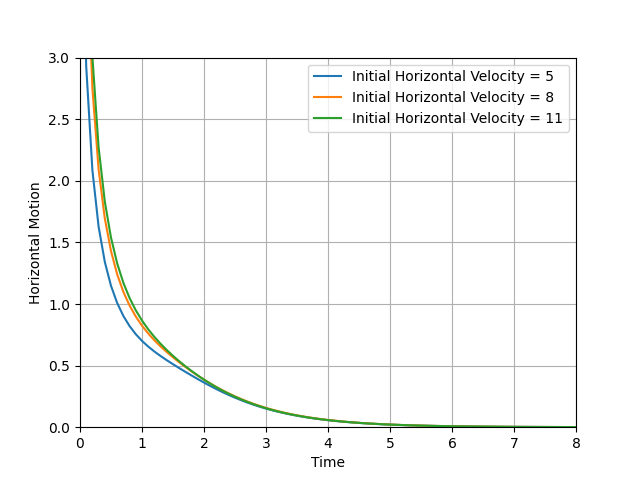
\includegraphics[width=0.6\textwidth]{figure1.png}
  \caption{\label{fig:figure1}
  Horizontal motion vs. time. 
  It is clear that the horizontal motion increases as its step is increased by 3.
  }
  \end{center}
\end{figure}

\begin{figure}[h!tbp]
  \begin{center}
 \item[]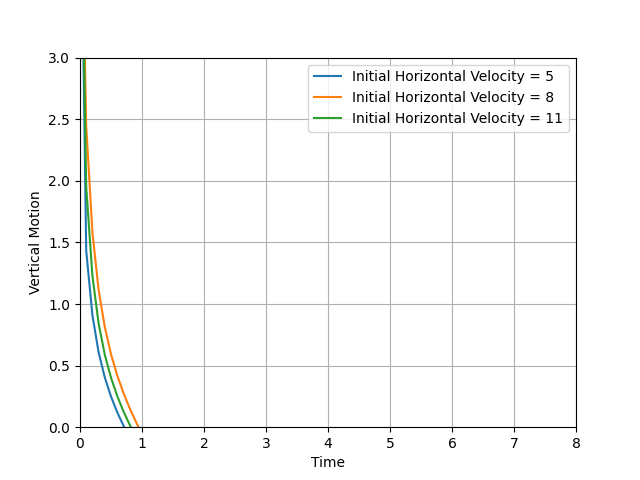
\includegraphics[width=0.6\textwidth]{figure2.png}
  \caption{\label{fig:figure2}
  Vertical motion vs. time. 
  The curve becomes increasingly shallow as the horizontal motion is increased.
  }
  \end{center}
\end{figure}

Changing the step in the horizontal motion can have effects in the vertical motion of the graph over time. 
This is directly based on the differential equations that model the motion. 
If the horizontal and vertical motion were independent, then changing the horizontal motion should not affect the vertical motion.

\pagebreak

\begin{center}
\subtitle{\textbf{Trajectories}}
\end{center}

The general shape of the projectile exhibits an parabolic shape based on the firing angle and the initial velocity. 
To find a relationship between the initial speed and launch angle, the horizontal and vertical components of velocity can be represented in terms of the launch angle and initial speed using the Pythagorean theorem.

\begin{equation} \label{eq:vocostheta}
  v_x = v_{0} \cos(\theta)
\end{equation}

\begin{equation} \label{eq:vosintheta}
  v_y = v_{0} \sin(\theta)
\end{equation}

Fig. \ref{fig:figure3} models the projectile against the vertical distance and horizontal distance at some initial angle and speed.

\begin{figure}[h!tbp]
  \begin{center}
 \item[]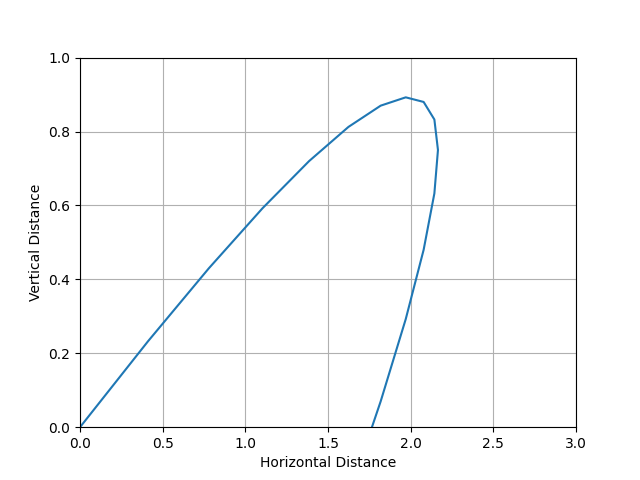
\includegraphics[width=0.6\textwidth]{figure3.png}
  \caption{\label{fig:figure3}
  General shape of the trajectory.
  }
  \end{center}
\end{figure}

The general shape of the projectile can change based on the initial speed and the initial angle. 
When the initial angle increases, the shape of the trajectory becomes steeper. 
The initial speed causes the projectile to go further when increased. 
The two figures below show this in greater detail with Figure \ref{fig:figure4} having the initial speed incremented by 0.5 and Figure \ref{fig:figure5} having an initial angle incremented by 10 degrees.

\begin{figure}[h!tbp]
  \begin{center}
 \item[]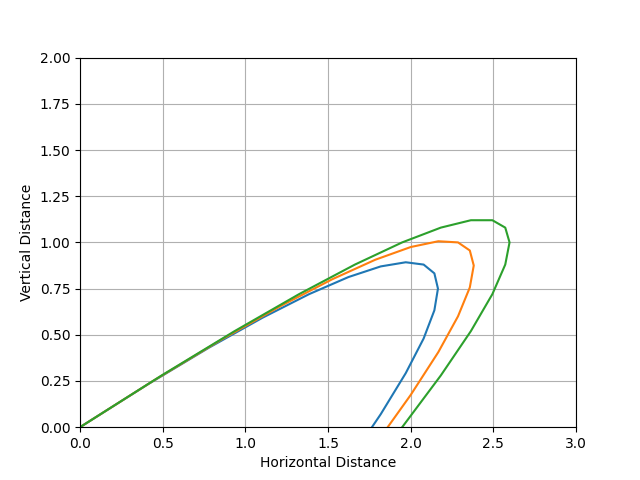
\includegraphics[width=0.6\textwidth]{figure4.png}
  \caption{\label{fig:figure4}
  Trajectory with an increasing initial speed.
  }
  \end{center}
\end{figure}

\begin{figure}[h!tbp]
  \begin{center}
 \item[]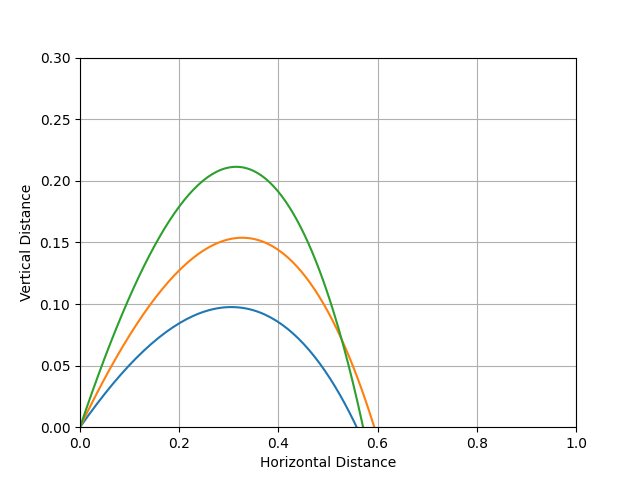
\includegraphics[width=0.6\textwidth]{figure5.png}
  \caption{\label{fig:figure5}
  Trajectory with an increasing initial angle.
  }
  \end{center}
\end{figure}

\pagebreak

\begin{center}
\subtitle{\textbf{Firing Range}}
\end{center}

To extract the range of the realistic projectile, we utilize the list feature in Python.
We will call the last number in the list of x values after the RK4 function has run.
It is important to note that the amount of x values can change depending on the parameters of the simulation, such as the angle of the launch, initial speed, gravitational acceleration, or drag constant.
This issue is avoided by calling the last item of the list by using the [-1] index.
This final x value is appended to a list that stores the final x value after each loop iteration.
A while loop is also needed so that the program can continue to run until we have our desired data sets, and we will utilize a counter to keep track of the value of our changing variable and to prevent the program from performing the same operations on a constant set of parameters.
We will then compare the range of the projectiles to our desired variable by creating a graph, and setting the range to the vertical axis so that the graph is a function of range, with respect to the variable of our choosing.

When analyzing the firing range as a function of firing angle for various fixed initial speeds, we found that there were two cases: when we are above or below terminal velocity.
When the projectile is above terminal velocity, it travels in a straight line until the projectile's velocity has decreased from drag.
Once the velocity has decreased enough to where it is below terminal velocity, gravity then pulls the object down until it eventually reaches the ground.
This behavior can be seen in Fig. \ref{fig:figure6}.


\begin{figure}[h!tbp]
  \begin{center}
 \item[]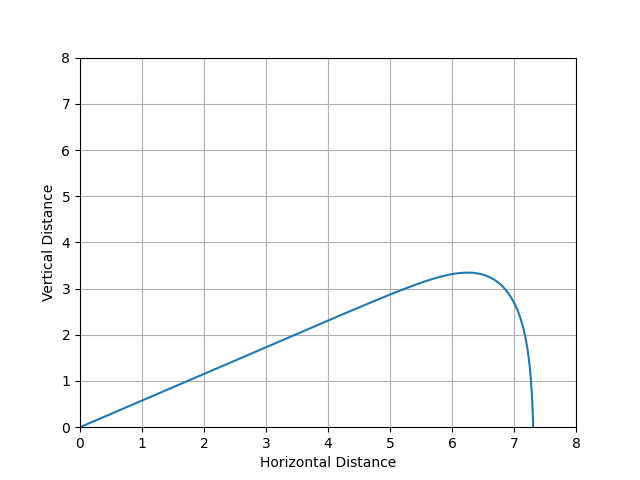
\includegraphics[width=0.6\textwidth]{figure6.png}
  \caption{\label{fig:figure6}
  Initial velocity of 2k with initial angle of 30 degrees.
  }
  \end{center}
\end{figure}

The amount of the trajectory that is linear is dependent on how high the initial velocity is set.
This means that the lower the initial angle, the further the projectile's range is, to a certain threshold.
At low enough angles, the range is shorter than some higher initial angles.
This can theoretically be avoided by having high enough speeds that enhance the effects of the drag force, but this is a limitation due to hardware.

When the initial velocity is below terminal velocity, the straight-line behavior of speeds greater than terminal velocity is not replicated.

\begin{figure}[h!tbp]
  \begin{center}
 \item[]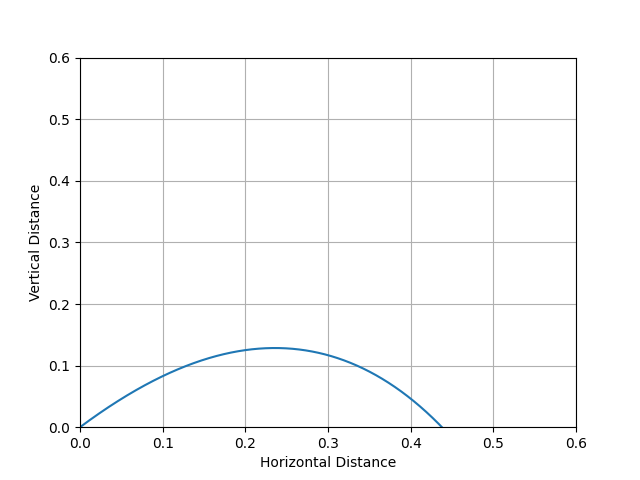
\includegraphics[width=0.6\textwidth]{figure8.png}
  \caption{\label{fig:figure8}
  $v_0 = 0.8$, initial angle is $\pi / 4$.
  Even with equal components of initial horizontal and vertical velocity, the graph is still not completely symmetrical.
  }
  \end{center}
\end{figure}

Since the shape of the graph is parabola-like and the horizontal and vertical components of motion are interdependent, the range is the greatest when both the horizontal and vertical components are the greatest, which is when the initial angle is $\pi / 4$, as in Fig. \ref{fig:figure8}.
With quadratic drag, we expect the range to decrease since drag increases with initial speed, and at the end of the projectile's trajectory, the vertical component is increasing in the downward direction due to gravity and the horizontal component has decreased relative to the initial launch.
This is why we see the "squished" shape of the trajectory.
Thus, for the greatest range we would look for a trajectory where the amount of drag is minimized, which is when the arc length is the shortest.

When the projectile's range is graphed against the initial angle with respect to the horizontal, we find that the shape of the curve is parabolic and concave down.

\begin{figure}[h!tbp]
  \begin{center}
 \item[]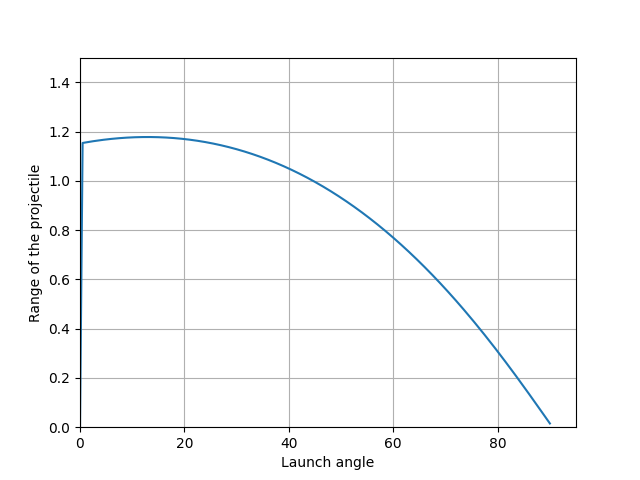
\includegraphics[width=0.6\textwidth]{figure7.png}
  \caption{\label{fig:figure7}
  Range as a function of the initial launch angle, with $v_0 = 1$.
  }
  \end{center}
\end{figure}


\pagebreak

%%%%%%%%%%%%%%%%%%%% Extension %%%%%%%%%%%%%%%%%%%%
\section{Extension: Incorporating Lift}

For the extension, we chose to incorporate a lift force that always points perpendicular to the velocity and, similar to the drag force, increases quadratically with velocity.
The lift force is defined by the equation:

\begin{equation} \label{eq:3}
  \vec{F_{L}} = m \Gamma |\vec{v}|
  \begin{pmatrix}
    -v_{y} \\
    v_{x}
  \end{pmatrix}

\end{equation}

This addition slightly modifies Eq. \ref{eq:1} and \ref{eq:2}, as there is now the lift constant, $\Gamma$, that controls the motion in both the horizontal and vertical directions.
Thus, these equations become:

\begin{equation} \label{eq:4}
  \frac{\mathrm{d}^2 x}{\mathrm{d}t^2} = -k v_x |\vec{v}| - \Gamma v_y |\vec{v}|
\end{equation}

\begin{equation} \label{eq:5}
  \frac{\mathrm{d}^2 y}{\mathrm{d}t^2} = g_y - k v_y |\vec{v}| + \Gamma v_x |\vec{v}|
\end{equation}

At each initial speed, there is an optimal lift constant that will maximize the range of the projectile.
If the lift constant is too high, it will cause the object to curve upwards, then shamefully fall back down to the ground.
If the lift constant is too low, the projectile's path bends downwards and undershoots the initial range.
These behaviors can be seen in Fig. \ref{fig:lift1}.

\begin{figure}[h!tbp]
  \begin{center}
 \item[]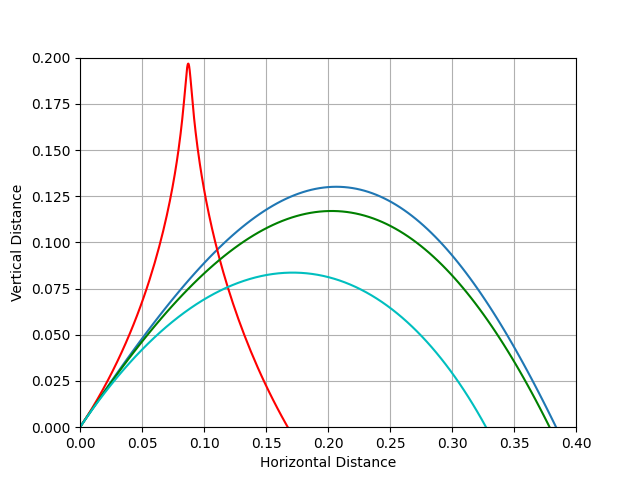
\includegraphics[width=0.6\textwidth]{lift1.png}
  \caption{\label{fig:lift1}
  Response of a projectile's trajectory with changing lift constant.
  All trajectories correspond to a launch angle of $\pi/4$ and $v_{x0} = v_{y0} = 0.5$.
  The blue trajectory corresponds to $\Gamma = 1$, red corresponds to $\Gamma = 5$, green corresponds to $\Gamma = 0.5$, and cyan corresponds to $\Gamma = -1$.
  }
  \end{center}
\end{figure}

As the projectile's initial speed increases, the optimal lift value decreases.
This is exhibited in Fig. \ref{fig:lift2}, where the lift constant is kept the same but the initial speed is changed.
At higher initial speeds, the projectile bends up earlier and loops, falling much earlier than it is supposed to.
This is expected, as the lift force's magnitude quadratically increases with speed, thus causing the projectile to bend backwards more dramatically on its climb upwards.

\begin{figure}[h!tbp]
  \begin{center}
 \item[]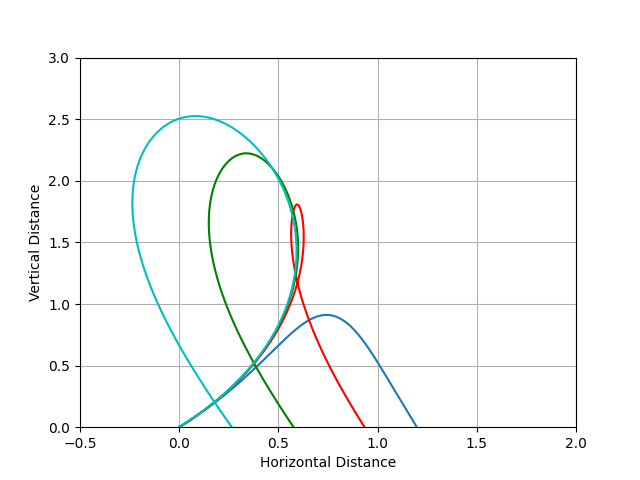
\includegraphics[width=0.6\textwidth]{lift2.png}
  \caption{\label{fig:lift2}
  Response of a projectile's trajectory with increasing initial speed while keeping the lift constant the same.
  All trajectories correspond to a launch angle of $\pi/4$ and $\Gamma = 0.5$.
  The blue trajectory corresponds to $v_{x0} = v_{y0} = 2$, red corresponds to $v_{x0} = v_{y0} = 5$, green corresponds to $v_{x0} = v_{y0} = 8$, and cyan corresponds to $v_{x0} = v_{y0} = 12$.
  }
  \end{center}
\end{figure}

With the lift constant high enough, the projectile will not only loop around but continue to glide as well.
In Fig. \ref{fig:lift3}, the projectile does a loop, peaks again, and then elegantly glides back down to the ground.
It is important to note that in each case tried with different initial speeds and lift constants, the projectile would hit the ground after the loop then emerge to peak again; thus, the projectile was given a starting height above the ground to prevent this from happening.

\begin{figure}[h!tbp]
  \begin{center}
 \item[]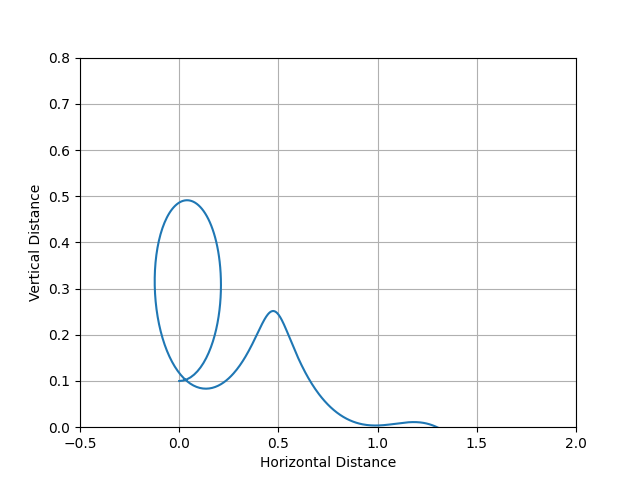
\includegraphics[width=0.6\textwidth]{lift3.png}
  \caption{\label{fig:lift3}
  Projectile "looping and gliding."
  Initial conditions are $v_{x0} = 2$, $v_{y0} = 0$, $y_{0} = 0.1$, and $\Gamma = 5$.
  }
  \end{center}
\end{figure}


\end{document}
%%%%%%%%%%%%%%%%%%%% Document Ends %%%%%%%%%%%%%%%%%%%%